\section{Second iteration: mobile and clarity redesign}
\label{sec:iteration2}

Iteration 2 answers the clearest iteration-1 finding: OSR was discovered on phones but built for desktops. One week after launch, between 18 and 24 June 2026, I redesigned the shipped site for small touchscreens (all dates below come from the repository history, archived in Drive \texttt{07 Development evidence}), then froze the redesign into a medium-fidelity click-through prototype and planned a five-task usability test against it.

\subsection{Design adjustments driven by iteration-1 evidence}

Each change traces to a coded launch theme or a PACT implication, and to dated commits.

\textbf{Viewport-fit single-column layout, no document scroll} (18 June 2026). The mobile theme (7 comments) reported layouts breaking and data never appearing on phones, and the PACT analysis had already named mobile the primary platform. Every page now lays out as a single column inside the visible viewport: panels scroll internally, the document itself never scrolls. Nothing important can sit below an edge the user does not know exists, and every state survives as a screenshot.

\textbf{A header that measures instead of guessing} (23 June 2026). The header measures whether its items fit the current width and collapses into a drawer (Material Design's navigation-drawer pattern \cite{materialdesign}) only when they do not, re-measuring on every window resize. I rejected a fixed breakpoint deliberately, because a threshold tuned on my own devices would relocate the breakage to devices I never tested, which is how the desktop-only launch failed in the first place.

\textbf{Pinch-zoom on the map and flow network} (18 June 2026). A direct answer to the most concrete mobile complaint: ``Opening it on my phone, it seems the map can't be zoomed?'' Two-finger zoom and pan now work on both the canvas map and the trajectory flow network, the two views that are useless at a fixed small scale.

\textbf{Touch-sized controls and occlusion fixes} (23 June 2026). Scale, bucket, and dimension controls grow to touch size when a coarse pointer is detected, following Material Design's touch-target guidance and the Fitts's-law link \cite{fitts1954} between target size and selection speed, and two commits remove panels overlapping content on the detail flow, the mobile about page, and the ranking pager at every width. Overlap on a 390-pixel-wide screen hides the values users came to read.

\textbf{Columns drop before rows} (24 June 2026). When a board runs out of width it drops whole columns in a fixed priority order (sort arrows first, city before country, cells stacking inside the columns that remain), and the dropped columns' filters stay reachable through a filter bar. Rows are never truncated. This is the clarity half of the redesign, and a visual-perception argument \cite{benyon}: a narrow board degrades into a smaller readable table whose type never shrinks below legibility, answering the legibility theme (6 comments) alongside the mobile one. The same day, the default landing route moved to \texttt{/mobility}, so a shared link opens directly on the board under evaluation. Figure~\ref{fig:mobile-redesign} contrasts the two form factors after the redesign: the same China-conditioned mobility view on a desktop and on a phone.

\begin{figure}[!t]
\centering
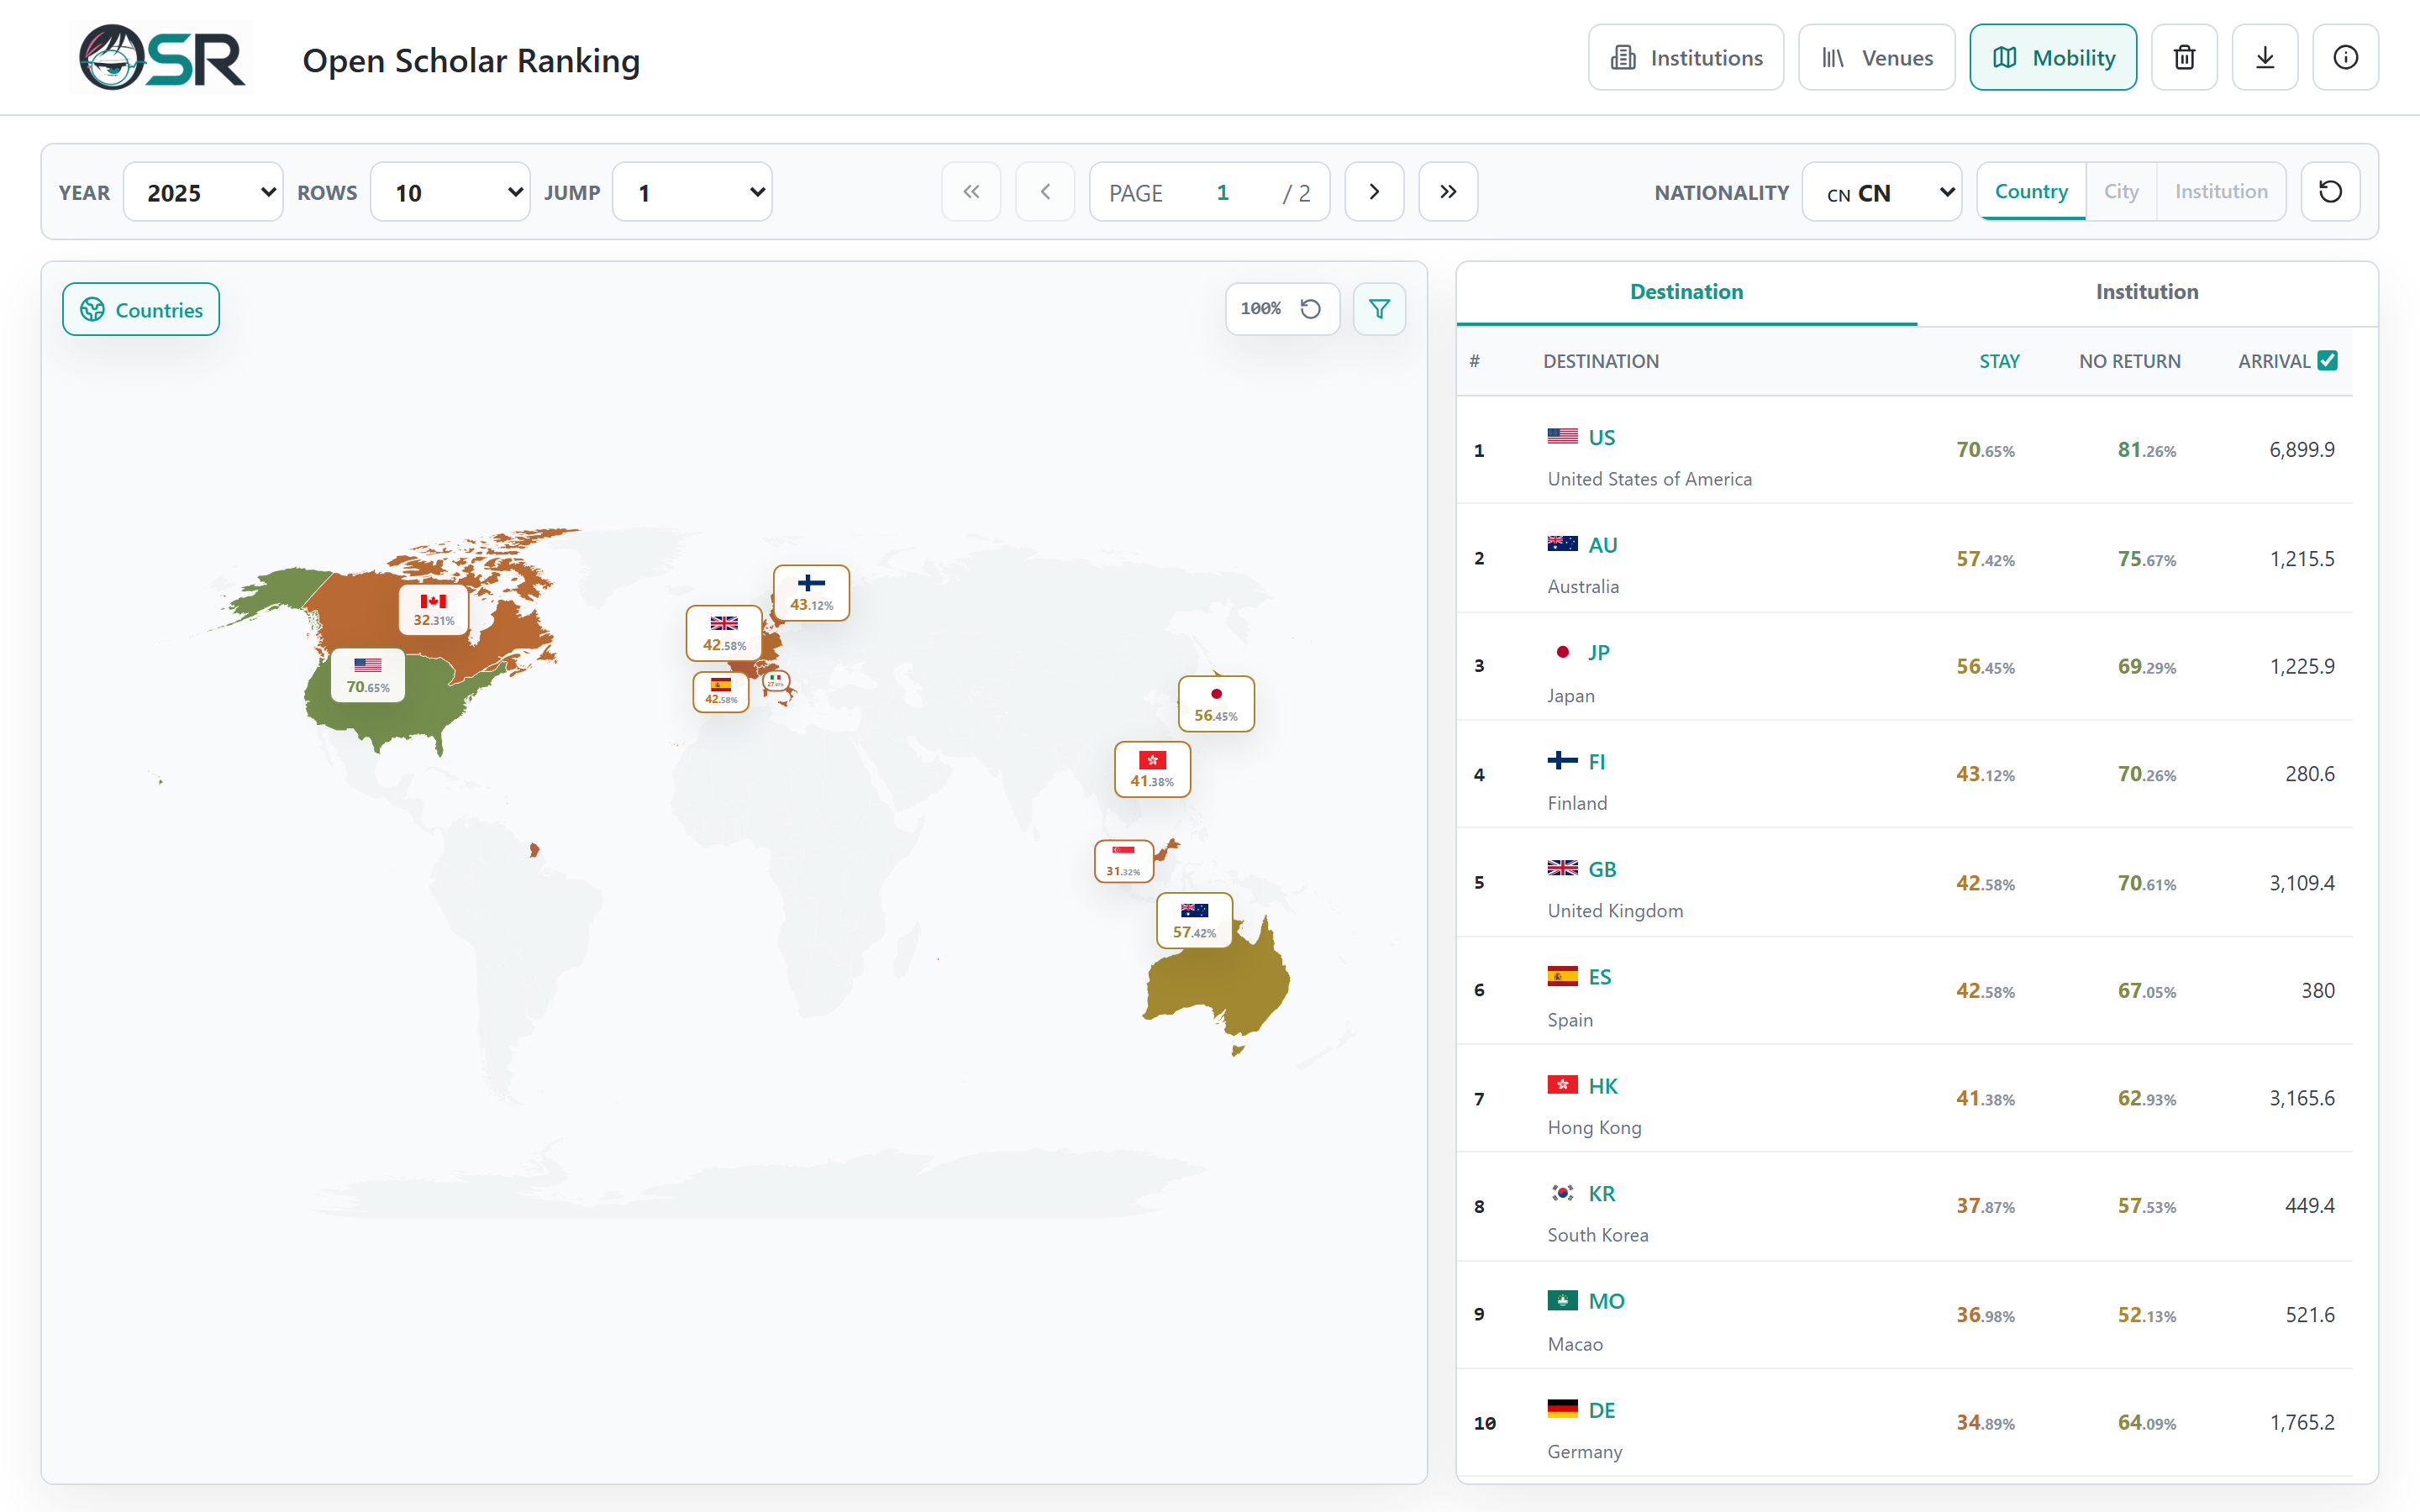
\includegraphics[width=0.60\linewidth]{figures/fig-mobility-cn}\hfill
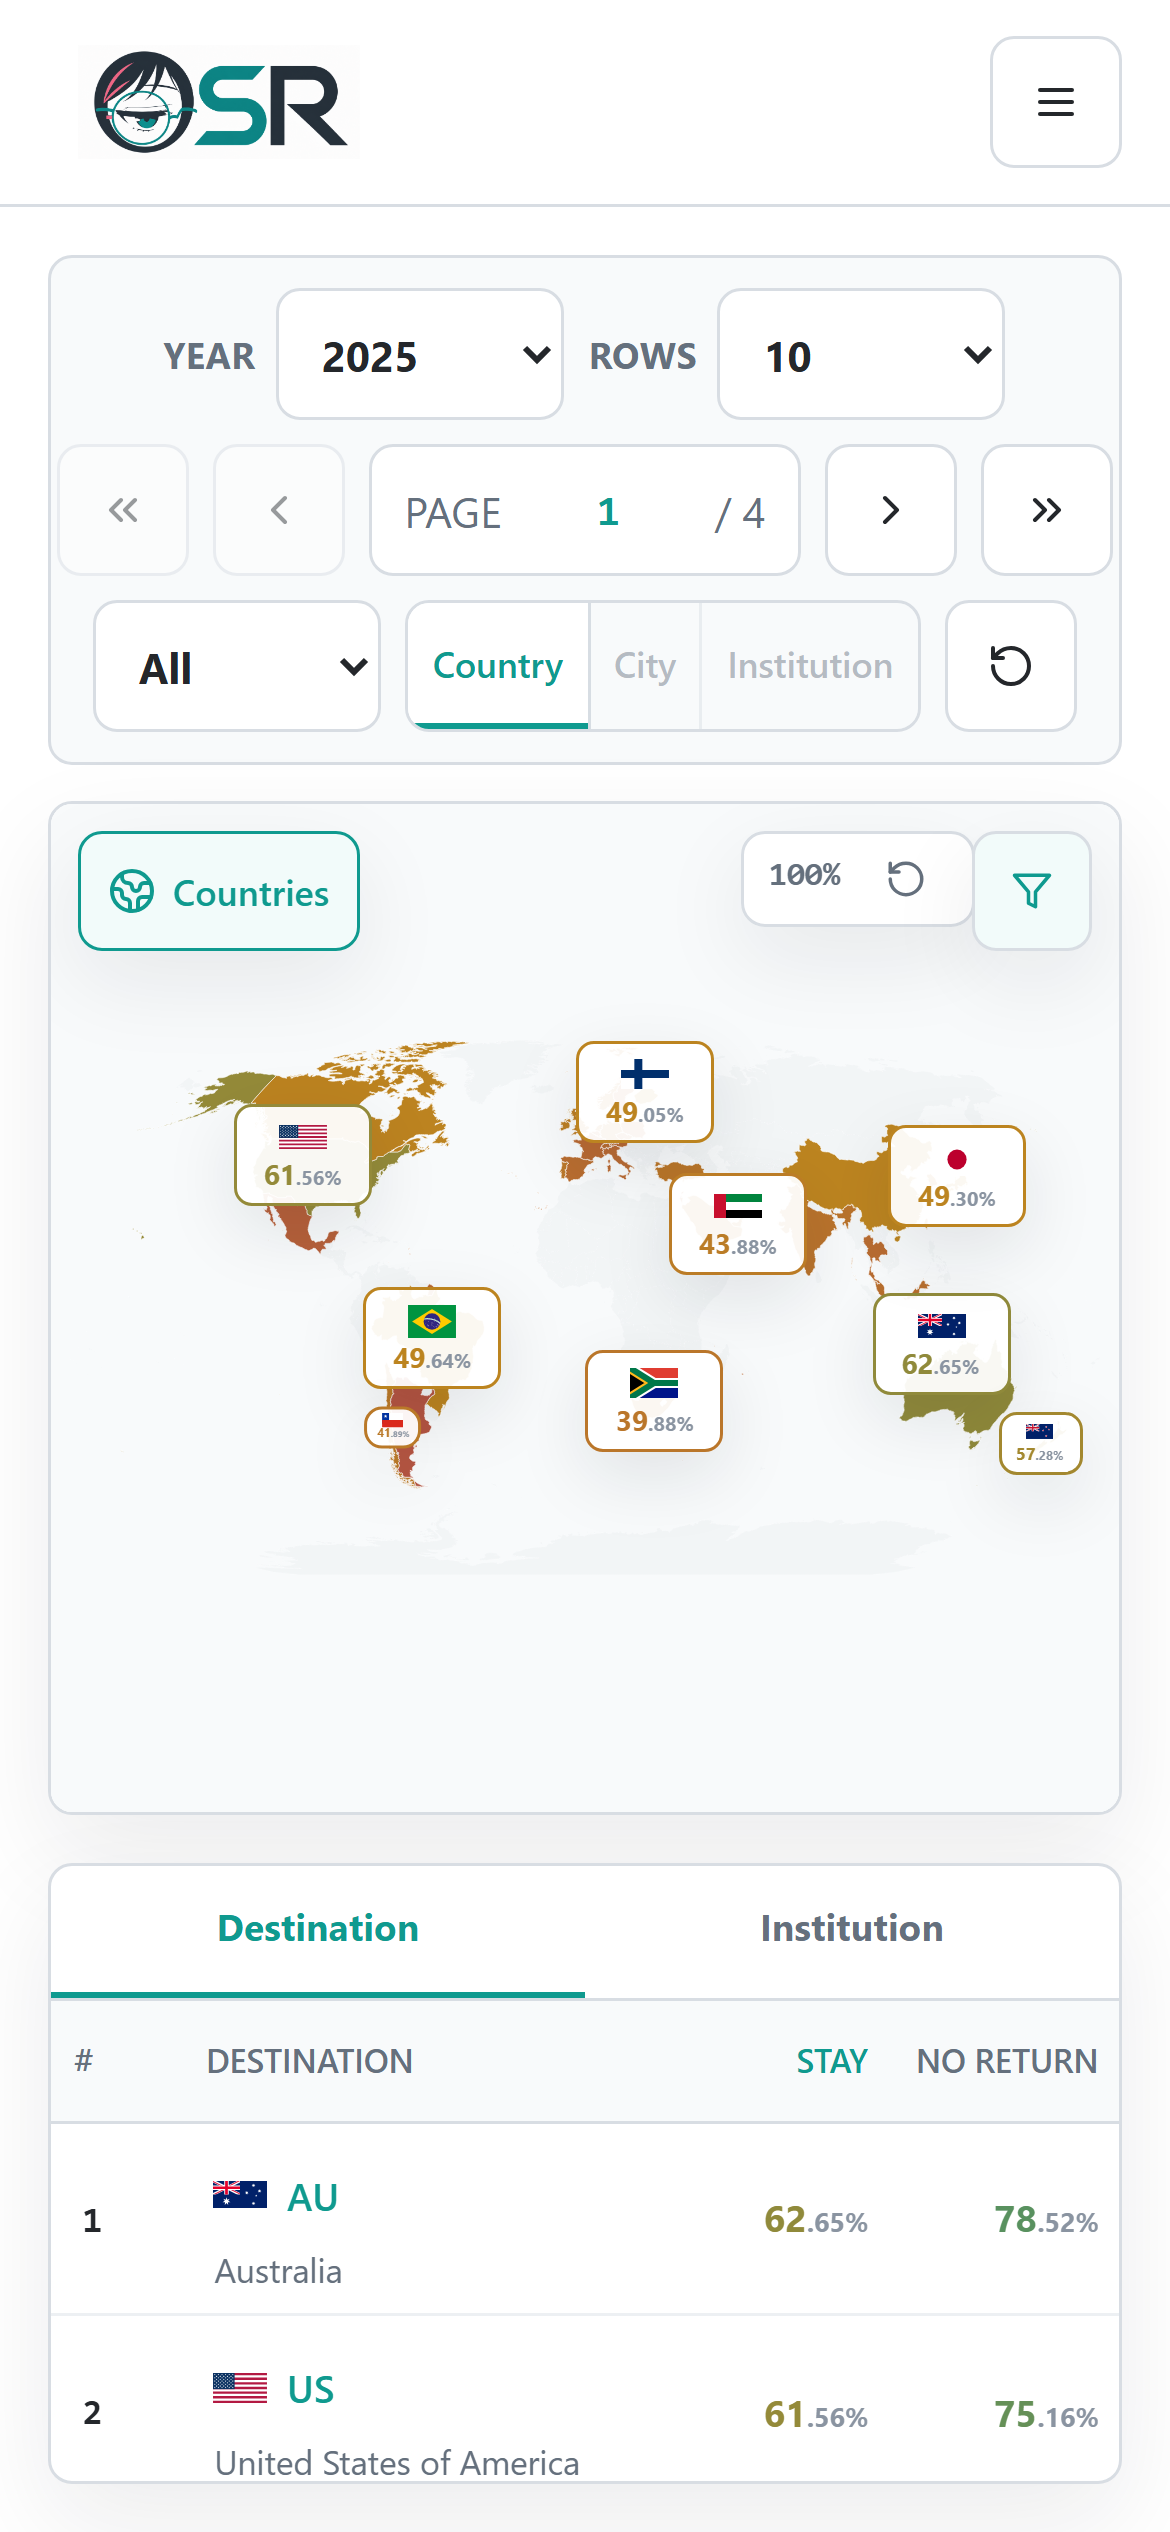
\includegraphics[width=0.275\linewidth]{figures/fig-mobility-mobile}
\caption{The redesigned mobility view with nationality CN, desktop (left) and phone (right): same data, one column (commits of 18--24 June 2026).}
\label{fig:mobile-redesign}
\end{figure}

\subsection{Prototyping}

For evaluation I needed a version of the redesign that participants could click through under controlled conditions. I assembled a medium-fidelity prototype in Axure RP 11 from full-page captures of the deployed redesign (file, cloud link, and assembly spec in Drive \texttt{02 Prototype}). Ten pages cover the evaluated paths: the mobility board, the board with nationality CN applied, the city layer after drilling into a country, the institution board with its R1--R4 tier chips (Figure~\ref{fig:institution-board}), the institution ranking with its detail pane, the methodology page, and two mobile captures reachable from a hub page. Three interactions are wired as real widgets rather than page links (the nationality droplist, the country/city granularity toggle, and the Destination/Institution board tabs), the three mechanisms the test tasks exercise. Every intentionally static control carries an annotation, so evaluators read dead regions as declared scope.

The fidelity pipeline is inverted here: the redesign was already deployed \cite{osr}, so the prototype is a frozen copy of the real interface and the deployed site is its implemented counterpart. What the prototype buys is control: a fixed data state, no network variance, and hotspot flashes that show participants where interactivity exists.

\begin{figure}[!t]
\centering
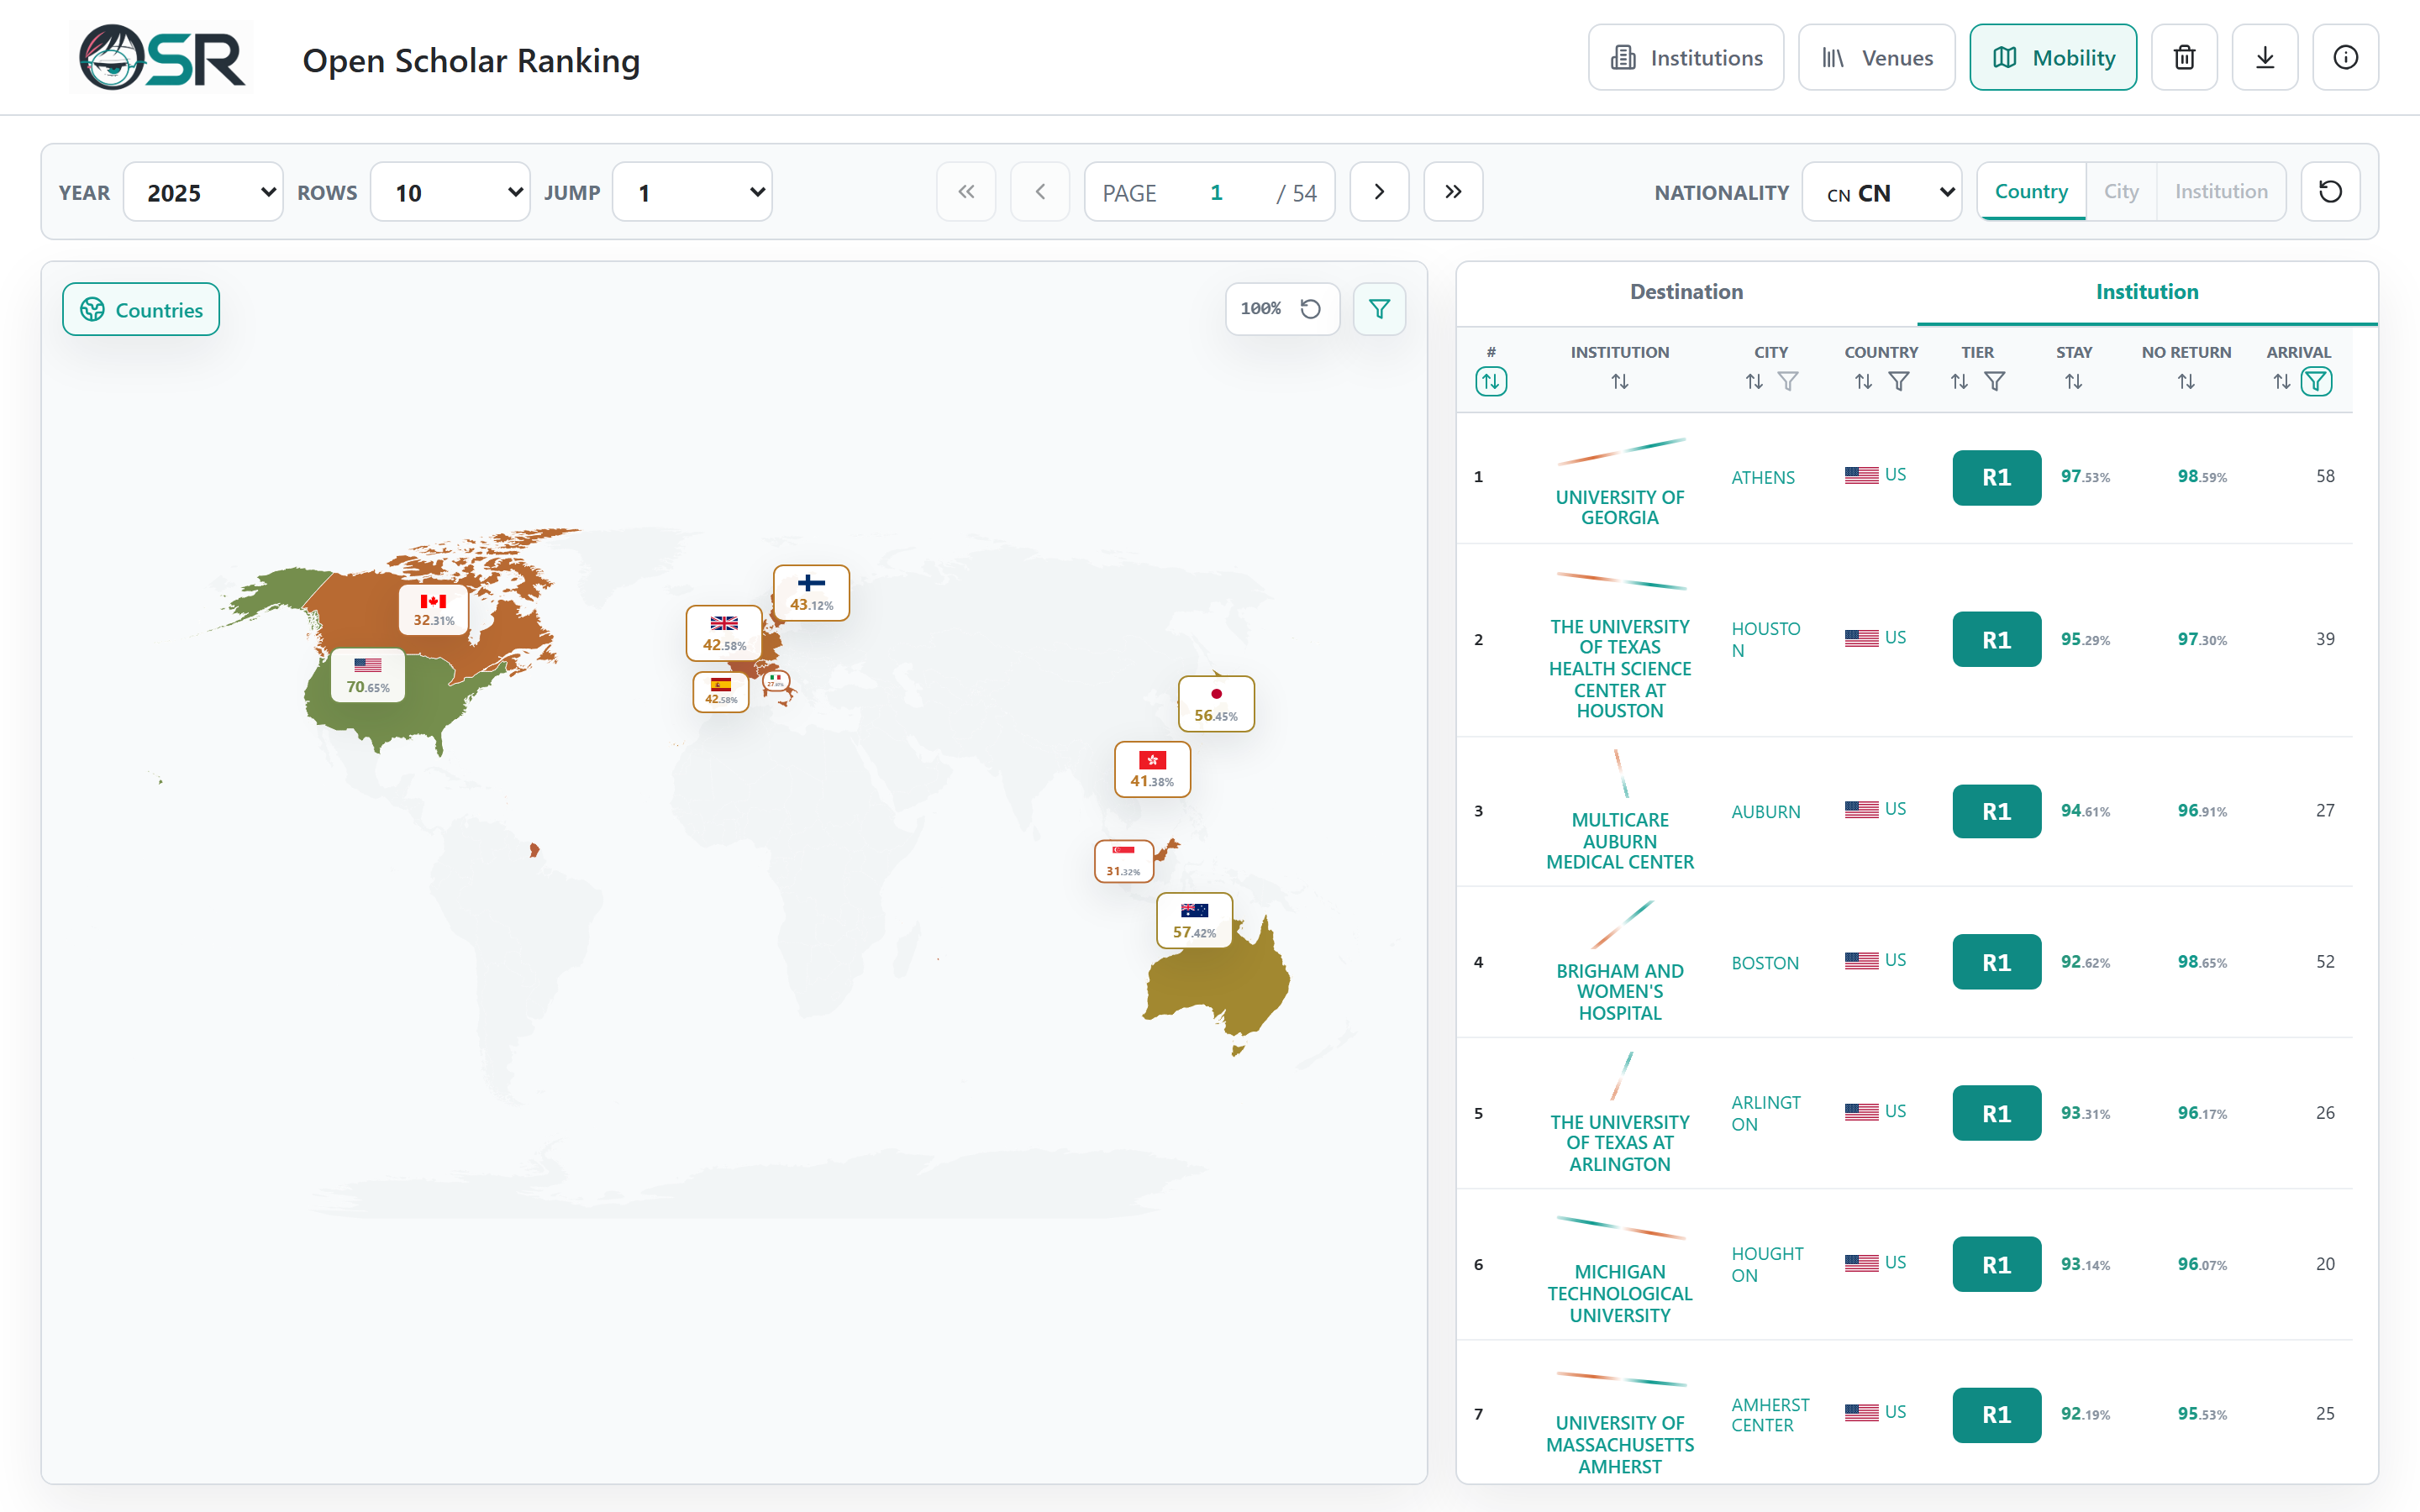
\includegraphics[width=0.72\linewidth]{figures/fig-institution-board}
\caption{The institution board with R1--R4 tier chips, one of the ten prototype pages.}
\label{fig:institution-board}
\end{figure}

\subsection{Evaluation: medium-fidelity usability test}

The second evaluation is a think-aloud usability test \cite{nielsen1993usability} with three participants against the prototype, run as the closing part of each combined session, one recording per participant: 25--35 minutes of testing, screen and audio recorded, protocol in Drive \texttt{05 Evaluations}. Tasks follow a fixed order, each with a success criterion and a time cap. T3 and T5 entered only in the third session as facilitation settled, so the first two sessions ran T1, T2, and T4:

\begin{enumerate}
\item Set the nationality filter to China and name the three countries with the highest Stay (3 min).
\item Switch to city granularity and name a top city in one of those countries (3 min).
\item On the institution board, find any university's tier and explain what R1 means (4 min).
\item Find the methodology page and state how Stay is defined (3 min).
\item Export the currently displayed board to a file (2 min).
\end{enumerate}

The tasks retrace the persona journeys: T1--T3 follow Chen Rui's shortlisting walk from country to city to institution, T4 is the trust-checking step that the metric-comprehension theme (14 comments) shows must precede belief, and T5 exercises the save-and-share loop. Export is one of the prototype's declared static regions, so T5 ran as identify-the-control. The participant had to locate the header's export affordance, and the fidelity cap is a validity limit on T5's timing and error data. Per participant and task I log success, assists (hints only after two minutes stuck, always logged), completion time, and errors. Afterwards each participant answers the ten-item SUS \cite{brooke1996sus} alone, then three open questions: the most confusing spot, the most useful spot for their real decision, and the single change they would make. At this sample size the SUS mean is only indicative.

Three sessions ran on 11--12 July 2026, all on desktop. The phone-width sessions the protocol called for did not happen, a deviation carried to the limitations. Table~\ref{tab:eval2} gives the task results. SUS came out at 90.0, 95.0, and 82.5 (mean 89.2) against the conventional benchmark of 68. The failures cluster in one layer, metric semantics. P02 paraphrased Stay as a time ratio rather than a person ratio (T4), P03 read the R1 tier as institutional influence rather than retention (T3), and the open answers added icon-only affordances. The methodology entry took P03 forty seconds to find (``not prominent''), and the export icon carries no label. The positives are as consistent: the shared-filter model read instantly for all three, two tried map countries as filters (a real demand, once a dead click), and the most-useful answers converged on the aggregation itself. P02 called it ``data scattered in many places, nobody doing this statistic''.

The pre-registered rule: any task failed by more than one participant, or a repeated error pattern, becomes the top fix; SUS below 68 reopens layout; open answers arbitrate. Applying it, no task failed twice, but metric-semantics misreadings recur across T3, T4, and participants. That repeated pattern makes point-of-use glosses (FR6) plus text labels on the icon-only controls the top fix. SUS sits far above 68; nothing at layout level reopens.

\begin{table}[!t]
\centering\small
\begin{tabular}{@{}lllll@{}}
\toprule
Task & Success & Assists & Median time (s) & Errors \\
\midrule
T1 nationality filter, top-3 Stay countries & 3/3 & 0 & 80 & 1 \\
T2 city granularity, top US cities & 3/3 & 1 & 45 & 1 \\
T3 institution tier, explain R1 & 0/1 & 0 & 50 & 1 \\
T4 methodology page, define Stay & 2/3 & 2 & 55 & 2 \\
T5 locate export control & 1/1 & 0 & 50 & 1 \\
\bottomrule
\end{tabular}
\caption{Usability-test results ($n=3$). T3/T5 reached only the third session; raw CSVs, recordings, and transcripts in Drive \texttt{05 Evaluations}. SUS: 90.0/95.0/82.5, mean 89.2.}
\label{tab:eval2}
\end{table}
